%課題研究レジュメテンプレート ver. 1.2

\documentclass[uplatex]{jsarticle}
\usepackage[top=20mm,bottom=20mm,left=20mm,right=20mm]{geometry}
\usepackage[T1]{fontenc}
\usepackage{txfonts}
\usepackage{wrapfig}
\usepackage[expert,deluxe]{otf}
\usepackage[dvipdfmx,hiresbb]{graphicx}
\usepackage[dvipdfmx]{hyperref}
\usepackage{pxjahyper}
\usepackage{secdot}


\makeatletter
  \renewcommand{\section}{%
    \if@slide\clearpage\fi
    \@startsection{section}{1}{\z@}%
    {\Cvs \@plus.5\Cdp \@minus.2\Cdp}% 前アキ
    {.5\Cvs \@plus.3\Cdp}% 後アキ
    %{\normalfont\Large\headfont\raggedright}}
    {\normalfont\raggedright}}

  \renewcommand{\subsection}{\@startsection{subsection}{2}{\z@}%
    {\Cvs \@plus.5\Cdp \@minus.2\Cdp}% 前アキ
    {.5\Cvs \@plus.3\Cdp}% 後アキ
    %{\normalfont\large\headfont}}
    {\normalfont}}

  \renewcommand{\subsubsection}{\@startsection{subsubsection}{3}{\z@}%
    {\Cvs \@plus.5\Cdp \@minus.2\Cdp}%
    {\z@}%
    %{\normalfont\normalsize\headfont}}
    {\normalfont}}
\makeatother
%ここから上を編集する必要はない.





\title{\vspace{-14mm}経常利益の予測と実数値}
\author{PMコース 矢吹研究室 1442020 大木崇雅}
\date{}%日付を入れる必要はない.
\pagestyle{empty}%ページ番号は振らない.
\begin{document}
\maketitle





\section{研究の背景}

1999年10月からインターネット上で株式のオンライントレードが可能になってから,株式がとても簡易に取引できるようになり普及が進んだ.株とは企業の資金調達のために発行している有価証券のことで,企業は投資家が株を買ってくれた資金を使って事業を拡大する.株を買うことは,株を発行している企業に出資して事業資金を提供していることを意味する.株価は企業が今後大きな利益を上げると期待できる要因があると大きく上場する.投資家は,今後の企業の成長性などに期待して株を買うが,その期待値の一つとして上がるのが,経常利益である.なぜなら経常利益は売り上げからコストを差し引いた営業利益に財務活動などの損益を加えた数値であり,企業全体の強さが色濃く表れているからである.営業利益とは売上高からコスト(人件費や材料費,広告宣伝費)などを差し引いたもので本業で稼いだ利益のことである.従って経常利益は本業と副業を合わせた会社の実力を示す利益を意味する\cite{BA67886013}.例え小規模企業でも,経常利益4億円を実現できれば,東京証券取引所や大阪証券取引所の市場2部への上場の資格を得ることができるため,経常利益は株式市場への影響力が大きいと思われる.

四季報には翌年の経常利益の予測も載っている.予測と実際の数値が長期的に近い数値の場合、東洋経済社の四季報は正確な予測ができているという可能性が高いため私は四季報に載っている経常利益から,企業の株価が予測できるのではないかと考えた.




\section{研究の目的}


本研究の目的は,四季報の出している経常利益の予測値と実際の数値との差が少ない企業の傾向を調べる事である.


\section{プロジェクトマネジメントとの関連}

プロジェクトマネージャーがどのような商品が売れているかを市場調査をする際に経常利益は1つの判断基準になると考えた.そのため経常利益の予測と実際の経常利益の推移を研究する.



\section{研究の方法}

東証一部に上場している約2000社の中から4分の1にあたる500社を調査しExcelに纏めて経常利益から得られる傾向を調べる.データは2016年現在東証一部に上場している会社の社名と銘柄コードをダウンロードして番号をランダムに振り,4で割り切れる番号の企業をExcelに打ち込む.年度ごとに企業の経常利益を出しているサイトは多くあったが,四季報の予測まで載せているホームページは殆どなかった.予測の情報が記載されているサイトはスキャンで取り込んだ画像データでpng状態で閲覧可能なサイトだったため,その年分のページを開いて画像データを視認してExcelに打ち込むという方法でデータを取得した.予測を折れ線,実際の数値を棒グラフの複合グラフにしてグラフを作った.

予測の数値を実際の経常利益の数値データで割った結果が1に近いほど正確な予測ができているものとし,割った数値全ての和から1991年から2016年までの26で割って平均を求めて1に近い数値の企業の傾向を調べた.

\section{研究の結果}
当初は500社を調べるつもりだったが計画的にデータを取得していなかったため,65社しかデータを取得できなかった.
経常利益の予測と,実際の経常利益との誤差が少ない傾向にあった会社は商社と国際運輸会社のどちらかの要素を含んでいる会社に多くみられた.名目上は電気機器メーカーの会社でも,商社も兼ね備えているという会社が多く,国外にも市場を展開しているという事がわかった.

以下の2社のモーターを作っている会社にも,予測と実際の経常利益との差が少ない傾向にあった.さらにこれらの会社は株価の値動きと,経常利益の動き方が似た傾向を示している事が判明した.やはり共通点は国外にも市場を展開しているという事だった.左が経常利益の予測と実際の数値で,右が株価である.

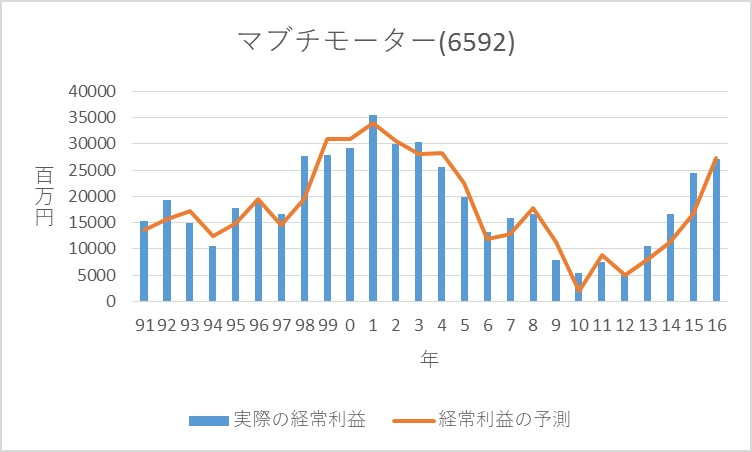
\includegraphics[width=8cm,height=7cm,bb=0 0 736 613]{mbt.jpg} 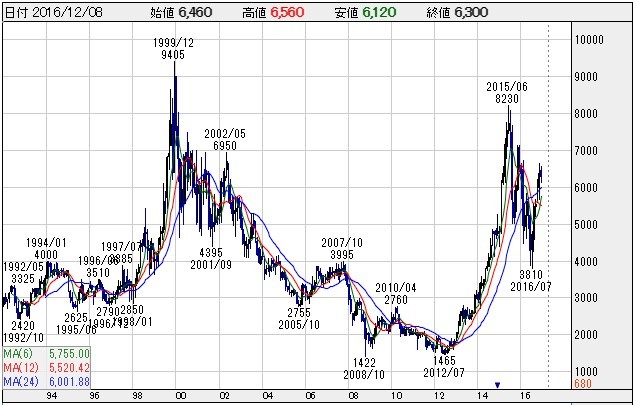
\includegraphics[width=8cm,height=7cm,bb=0 0 636 406]{mbtkbk.jpg}
\cite{self}\\
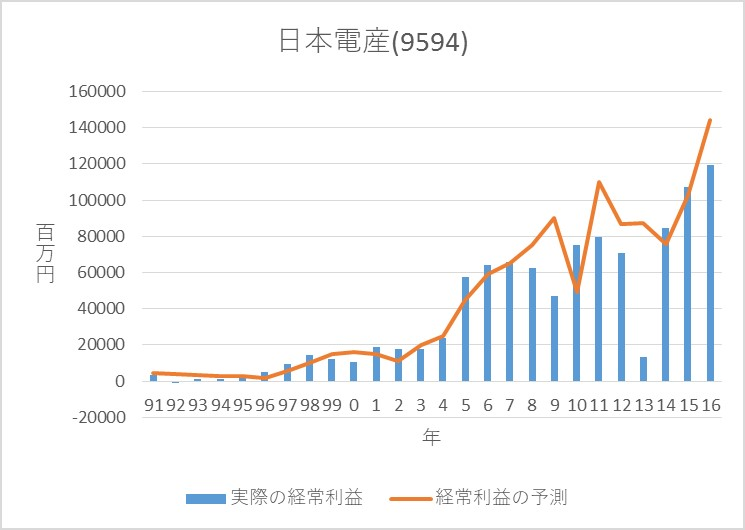
\includegraphics[width=8cm,height=7cm,bb=0 0 745 530]{densan.jpg} 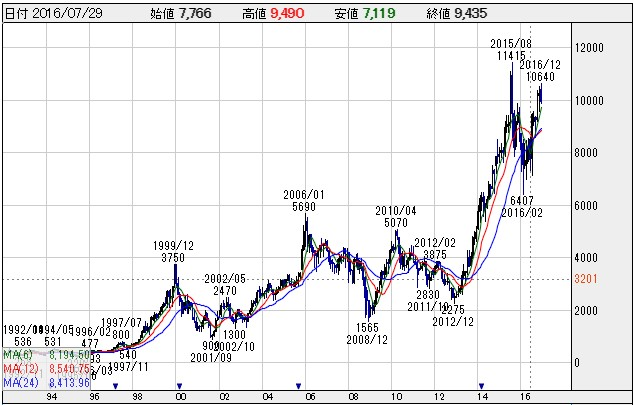
\includegraphics[width=8cm,height=7cm,bb=0 0 634 405]{densankbk.jpg}
\cite{sasa}\\



\section{今後の計画}
現在の65社のサンプル数では少なすぎるので,目標の500社に届くようにサンプル数を増やしてより説得力のあるデータを作るため,今後以下のように研究を進める.
\begin{enumerate}
\item ディープラーニングのように自動的に画像データから文字を読み取れるプログラムを作成し,データの取得効率を上げる.
\item 取得したデータを自動でグラフ化するプログラムを作成する.
\end{enumerate}

\bibliographystyle{junsrt}
\bibliography{biblio}%「biblio.bib」というファイルが必要.

\end{document}